\documentclass[letter,11pt]{article}
\usepackage{hyperref}
\usepackage{graphicx}
\usepackage{fancyhdr}
\usepackage{float} % Force figure placement
\usepackage{multicol}
\pagestyle{fancy}
\usepackage[letterpaper, margin=1in]{geometry}
\geometry{letterpaper}
\usepackage{parskip} % Disable initial indent

\usepackage[utf8]{inputenc}
\fancyhf{}
\renewcommand{\headrulewidth}{0pt} % Remove default underline from header package
\rhead{CYBR/CMSC 691 - Lab 9}
%\rhead{}
\lhead{\begin{picture}(0,0) \put(0,-10){
\includegraphics[width=1.1cm]{Images/UMBC-vertical}} \end{picture}}
\cfoot{\thepage}
\rfoot{Spring 2020}
\lfoot{Lab 9}
%\AtEndDocument{\vfill \hfill \LaTeX}

\begin{document}

\section*{Lab 9: Malware Feature Importance}
\paragraph{}Revisit the code from Lab 4 where you created models. Using the Python package \texttt{shap}, identify which features were more important to your model. Decide on which features to add to your model, and which to remove.

\textbf{Points:} 40

\begin{figure}[H]
    \centering
    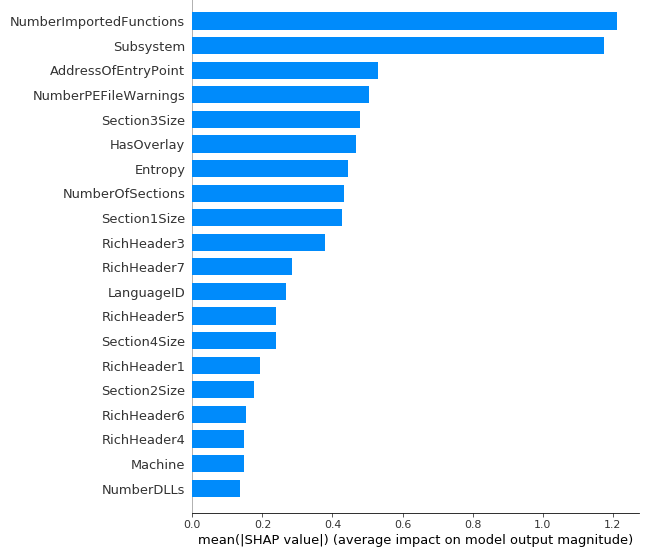
\includegraphics[scale=0.5]{Images/Lab9_shap_example.png}
    \caption{Shap example showing feature importance}
\end{figure}

\section*{Questions}
\paragraph{}In a separate document, provide your answers to the following questions. The expected format is a Word document, or similar, with a few images demonstrating your progress. The assignment will be submitted via Blackboard.

\begin{itemize}
    \item Which features were useful for making the malware vs. goodware decision?
    \item Which features were not helpful?
    \item Where there any surprises? Is this what you expected?
    \item What was your prior model's performance, and how much improvement have you gained?
\end{itemize}
\end{document}